\section{Question 1}

\subsection{Data Preprocessing}

We first import the data from the .csv file. Our data contains 398 observations, 9 columns including mpg, cylinders, displacement, horsepower, weight, acceleration, model$\_$year, origin, car$\_$name. 

Before we could use this data, we need to check for a few problem:

\subsubsection{Missing data}

There is some observation with horsepower column missing, this is denoted by the character "?" in our data set. We need to remove these before we can continue working on this data set. After removing them, we are left with 392 observations.

\subsubsection{Outlier}

We then have to check for outlier data of the data set. Here is the box plot for mpg.

\begin{figure}[H]
\centering
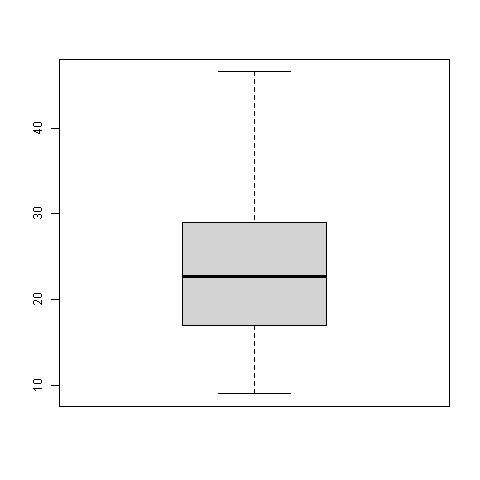
\includegraphics[scale=0.4]{img/mgpboxplot.png}
\caption{Box plot of mpg}
\label{fig:box_plot_mpg}
\end{figure}

So, there is no outlier in our data set. This can be validated by using the data in the summary of the data set in the next section, where all data point value deviate no more than 3 time the standard error from the mean.

\subsection{Data overview}

Here is the basic univariate summary statistics for our variables. 

\begin{center}
\begin{minipage}{\linewidth}
\begin{center}
  \captionof{table}{Basic univariate summary statistics for the continuous quantitative variables}
\begin{tabular}{lrrrrrrrrrr}
  \toprule
   & N &   & Mean & SD &   & Min & Q1 & Median & Q3 & Max \\ 
    \cmidrule{2-2}  \cmidrule{4-5} \cmidrule{7-11}
  mpg & 392 &  & 23.45 & 7.81 &  & 9.00 & 17.00 & 22.75 & 29.00 & 46.60 \\ 
  displacement & 392 &  & 194.41 & 104.64 &  & 68.00 & 105.00 & 151.00 & 284.50 & 455.00 \\ 
  horsepower & 392 &  & 104.47 & 38.49 &  & 46.00 & 75.00 & 93.50 & 127.00 & 230.00 \\ 
  weight & 392 &  & 2977.58 & 849.40 &  & 1613.00 & 2224.50 & 2803.50 & 3616.50 & 5140.00 \\ 
  acceleration & 392 &  & 15.54 & 2.76 &  & 8.00 & 13.75 & 15.50 & 17.05 & 24.80 \\ 
   \bottomrule
\end{tabular}
\end{center}
\end{minipage}
\end{center}

\begin{center}
\begin{minipage}{\linewidth}
\begin{center}
  \captionof{table}{Basic univariate summary statistics for model$\_$year}
\begin{tabular}{llrrr}
  \toprule
   & Level &   & N & \% \\ 
    \cmidrule{2-2} \cmidrule{4-5} 
 model\_year & 70 &  &  29 & 7.4 \\ 
   & 71 &  &  27 & 6.9 \\ 
   & 72 &  &  28 & 7.1 \\ 
   & 73 &  &  40 & 10.2 \\ 
   & 74 &  &  26 & 6.6 \\ 
   & 75 &  &  30 & 7.7 \\ 
   & 76 &  &  34 & 8.7 \\ 
   & 77 &  &  28 & 7.1 \\ 
   & 78 &  &  36 & 9.2 \\ 
   & 79 &  &  29 & 7.4 \\ 
   & 80 &  &  27 & 6.9 \\ 
   & 81 &  &  28 & 7.1 \\ 
   & 82 &  &  30 & 7.7 \\ 
   \bottomrule
\end{tabular}
\end{center}
\end{minipage}
\end{center}

\begin{center}
\begin{minipage}{\linewidth}
\begin{center}
  \captionof{table}{Basic univariate summary statistics for origin}
\begin{tabular}{llrrr}
  \toprule
   & Level &   & N & \% \\ 
    \cmidrule{2-2} \cmidrule{4-5} 
 origin & 1 &  & 245 & 62.5 \\ 
   & 2 &  &  68 & 17.3 \\ 
   & 3 &  &  79 & 20.2 \\ 
   \bottomrule
\end{tabular}
\end{center}
\end{minipage}
\end{center}

\begin{center}
\begin{minipage}{\linewidth}
\begin{center}
  \captionof{table}{Basic univariate summary statistics for cylinders}
\begin{tabular}{llrrr}
  \toprule
   & Level &   & N & \% \\ 
    \cmidrule{2-2} \cmidrule{4-5} 
 cylinders & 3 &  &   4 & 1.0 \\ 
   & 4 &  & 199 & 50.8 \\ 
   & 5 &  &   3 & 0.8 \\ 
   & 6 &  &  83 & 21.2 \\ 
   & 8 &  & 103 & 26.3 \\ 
   \bottomrule
\end{tabular}
\end{center}
\end{minipage}
\end{center}

\subsection{Data splitting}

The data is split into two part, training dataset and validation dataset. Training dataset contains 80$\%$ of the observations and the validation dataset contains 80$\%$ of the observations. The split is performed randomly with RStudio.

For replication, we use the seed 0.

\subsection{Model building}

\subsubsection{Response}

Fuel efficiency, calculated as miles per gallon (mpg), is the target output of our model. The mpg values for each car are positive real numbers. The following histogram illustrates the spread of fuel efficiency across our dataset.

\begin{figure}[H]
\centering
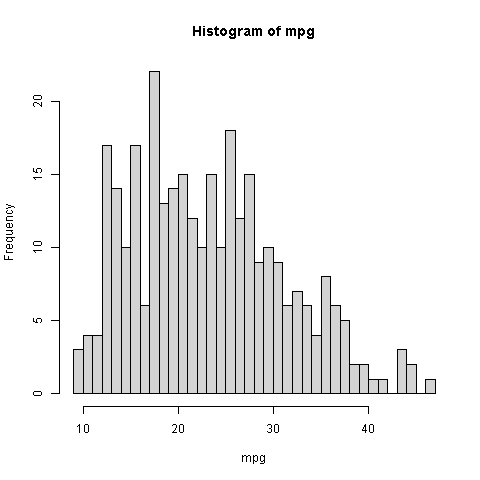
\includegraphics[scale=0.55]{img/mpghist.png}
\caption{Histogram of mpg}
\label{fig:hist_of_mpg}
\end{figure}

As the histogram clearly shown, the data is skewed to the right. We will fix this in a later section.

\subsubsection{Predictor}

\begin{itemize}
    \item Cylinders value for each car is a positive number which denote the number of cylinders in our car. Here is the bar plot for cylinders:

\begin{figure}[H]
\centering
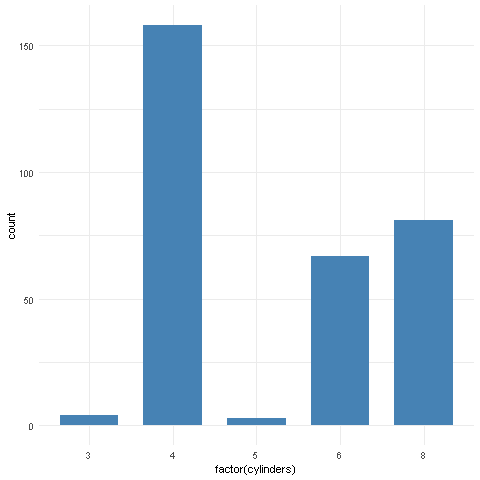
\includegraphics[scale=0.55]{img/cylinderbarplot.png}
\label{fig:cylinder_bar_plot}
\end{figure}

    \item Displacement is a continous variable in our dataset. It is the size of the engine of the car. Here is a histogram of it:

\begin{figure}[H]
\centering
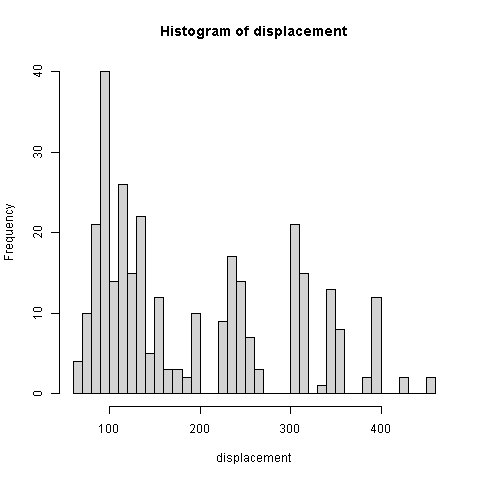
\includegraphics[scale=0.55]{img/disphist.png}
\caption{Histogram of displacement}
\label{fig:histogram_of_displacement}
\end{figure}

    \item The engine's horsepower reflects how much power the car can produce. It is an important indicator of performance, particularly for sports and high-performance vehicles. Here is the histogram showing the distribution of horsepower across the dataset:

\begin{figure}[H]
\centering
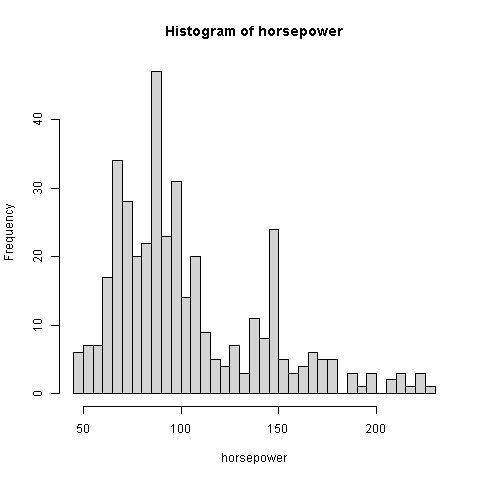
\includegraphics[scale=0.55]{img/hphist.png}
\caption{Histogram of horsepower}
\label{fig:horsepower_histogram}
\end{figure}

    \item Weight measures how heavy each car is. Heavier cars tend to have higher fuel consumption but can also offer more stability. Below is the histogram illustrating the distribution of car weights in our dataset:

\begin{figure}[H]
\centering
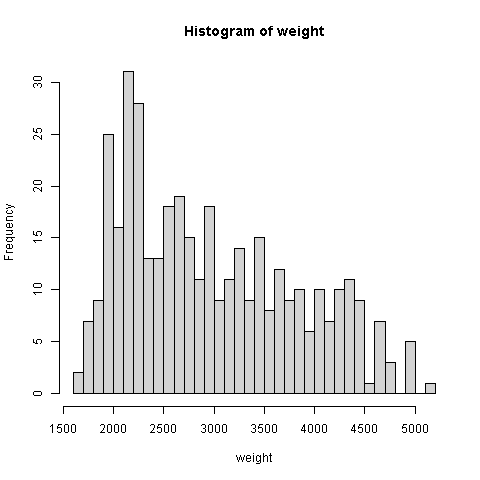
\includegraphics[scale=0.55]{img/weighthist.png}
\caption{Histogram of weight}
\label{fig:weight_histogram}
\end{figure}

    \item Acceleration represents the time taken by the car to reach a certain speed from a standstill. Cars with better acceleration offer quicker response and can handle rapid speed changes more effectively. Here is a histogram of the acceleration values:

\begin{figure}[H]
\centering
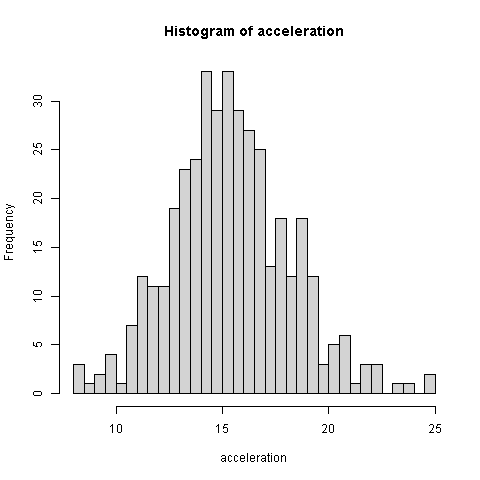
\includegraphics[scale=0.55]{img/accelhist.png}
\caption{Histogram of acceleration}
\label{fig:acceleration_histogram}
\end{figure}

    \item The model year provides insights into when the car was manufactured. Over time, car designs and technologies have evolved, and the model year can reflect those changes. The bar plot below shows the distribution of model years in the dataset:

\begin{figure}[H]
\centering
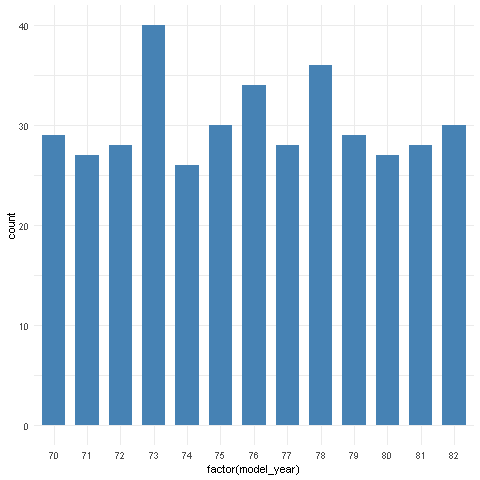
\includegraphics[scale=0.4]{img/modelyearbarplot.png}
\caption{Barplot of model$\_$year}
\label{fig:model_year_barplot}
\end{figure}

    \item Origin indicates the geographical region where the car was manufactured. This dataset categorizes cars by their origins as North America (1), Europe (2), and Asia (3). The bar plot below shows how the cars are distributed across these regions:

\begin{figure}[H]
\centering
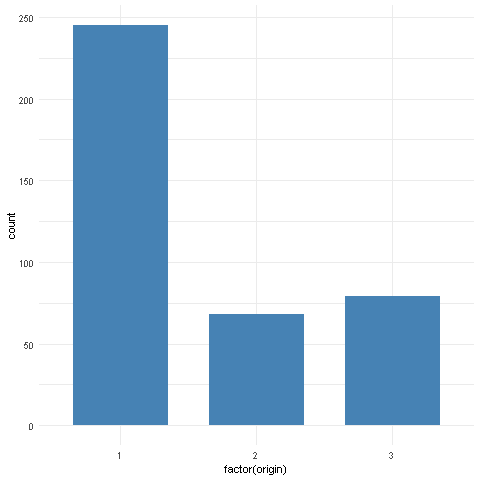
\includegraphics[scale=0.4]{img/originbarplot.png}
\caption{Origin barplot}
\label{fig:origin_barplot}
\end{figure}


\end{itemize}

\subsubsection{Model selection method}

We use the stepwise method as it is a simple, easy to implement and effective method for model selection. It combines both forward and backward selection, adding and removing predictors iteratively until no further improvement is observed.

\subsubsection{Evaluation parameter}

The model built should be evaluate using the following parameter:

\begin{itemize}
    \item $R^2$: It helps us assess the overall fit of your model. A higher R-squared generally implies a better fit
    \item Adjusted $R^2$: As we add more independent variables to a model, R-squared will always increase or stay the same, even if the added variables are not significant. Adjusted R-squared accounts for this by penalizing the model for adding unnecessary variables
    \item AIC and BIC, AIC is mainly use to perform stepwise procedure. These parameter is similar to adjusted $R^2$ as they imposed a penalty on complex model.
    \item Sharpio-Wilk test p-value, this is used to determine whether a sample of data comes from a normally distributed population. This is crucial if we want to do ANOVA or t-test with our result model.
    \item Durbin-Waston test value, this determine whether the residuals of a regression model are correlated with each other. This violates one of the key assumptions of linear regression, which is that the errors are independent as this may lead to inaccuracy in our model.
    \item Levene test p-value, this check the assumption of homogeneity of variance. This assumption is crucial for many statistical tests, particularly ANOVA and t-tests.
\end{itemize}

\subsubsection{Baseline model}

Our first model is just taking the linear model of mpg as response and all other 7 variables as linear predictor.

So our first model will take the forms of:

\begin{center}
$
mpg \ = \ \beta_1 \ + \ \beta_2 \ cylinders \ + \ \beta_3 \ displacement \ + \ \beta_4 \ horsepower \ + \ \beta_5 \ weight \ + \ \beta_6 \ acceleration \ + \ \beta_7 \ model\_year \ + \ \beta_8 \ origin \ + \ \epsilon
$
\end{center}

We run this model in R and obtain the result:

\begin{table}[H]
\centering
\captionof{table}{Summary of model parameter in R}
\begin{tabular}{rrrrr}
  \hline
 & Estimate & Std. Error & t value & Pr($>$$|$t$|$) \\ 
  \hline
(Intercept) & -19.5296 & 5.2529 & -3.72 & 0.0002 \\ 
  cylinders & -0.1863 & 0.3794 & -19 & 0.6237 \\ 
  displacement & 0.0125 & 0.0089 & 1.40 & 0.1612 \\ 
  horsepower & -0.0167 & 0.0157 & -1.06 & 0.2889 \\ 
  weight & -0.0063 & 0.0007 & -8.48 & 0.0000 \\ 
  acceleration & 0.1274 & 0.1123 & 1.13 & 0.2573 \\ 
  model\_year & 0.7652 & 0.0585 & 13.08 & 0.0000 \\ 
  origin & 1.3138 & 0.3217 & 4.08 & 0.0001 \\ 
   \hline
\end{tabular}
\\[0.5cm]
Residual standard error: 3.454 on 305 degrees of freedom
\\
Multiple R-squared:  0.8131,	Adjusted R-squared:  0.8088
\\
F-statistic: 189.5 on 7 and 305 DF,  p-value: < 2.2e-16
\end{table}

There is a few change we can make to our model:

\begin{itemize}
    \item cylinders: It's p-value is very high, and it's likely that it does not have a statistical significance to our model.
    \item Displacement: It's p-value is very high, and it's likely that it does not have a statistical significance to our model.
    \item Horsepower: It's p-value is very high, and it's likely that it does not have a statistical significance to our model.
    \item Acceleration: It's p-value is very high, and it's likely that it does not have a statistical significance to our model.
    \item Origin: It represent the production region of the car (Asia, North America, Europe) as such, it reasonable for it to not have a linear relation to our model.
    \item Model$\_$year: It represent the year that the car is manufactured. While it's reasonable for car manufactured technique to become better, the change may not be linear. \footnote{We do not try to evaluate this variable as a qualitative variable, even though it may improved the accuracy of our model. We will explain this at a later chapter}
\end{itemize}

Firstly, we can make indicator variable for origin, the resulting model will be:

\begin{center}
$
mpg \ = \ \beta_1 \ + \ \beta_2 \ cylinders \ + \ \beta_3 \ displacement \ + \ \beta_4 \ horsepower \ + \ \beta_5 \ weight \ + \ \beta_6 \ acceleration \ + \ \beta_7 \ model\_year \ + \ \beta_8 \ origin_2 \ + \ \beta_9 \ origin_3 \ + \ \epsilon
$
\end{center}

Other variable with little statistical significance will be removed later after we perform the stepwise procedure, so no need to removing them now.

Putting this model through R provide us with the following result:

\begin{table}[H]
\centering
\captionof{table}{Summary of the second model parameter in R}
\begin{tabular}{rrrrr}
  \hline
 & Estimate & Std. Error & t value & Pr($>$$|$t$|$) \\ 
  \hline
(Intercept) & -21.0709 & 5.2560 & -4.01 & 0.0001 \\ 
  cylinders & -0.2000 & 0.3751 & -0.53 & 0.5943 \\ 
  displacement & 0.0170 & 0.0089 & 1.91 & 0.0573 \\ 
  horsepower & -0.0166 & 0.0155 & -1.07 & 0.2850 \\ 
  weight & -0.0066 & 0.0007 & -8.84 & 0.0000 \\ 
  acceleration & 0.1216 & 0.1110 & 1.10 & 0.2740 \\ 
  model\_year & 0.7990 & 0.0590 & 13.54 & 0.0000 \\ 
  origin2 & 2.9302 & 0.6493 & 4.51 & 0.0000 \\ 
  origin3 & 2.5944 & 0.6360 & 4.08 & 0.0001 \\ 
   \hline
\end{tabular}
\\[0.5cm]
Residual standard error: 3.414 on 304 degrees of freedom 
\\
Multiple R-squared:  0.818,	Adjusted R-squared:  0.8132
\\
F-statistic: 170.7 on 8 and 304 DF,  p-value: < 2.2e-16
\end{table}

Then, we perform the stepwise regression technique on this model to obtain our baseline:

\begin{table}[H]
\centering
\captionof{table}{Summary of the baseline model parameter in R}
\begin{tabular}{rrrrr}
  \hline
 & Estimate & Std. Error & t value & Pr($>$$|$t$|$) \\ 
  \hline
(Intercept) & -23.7380 & 4.7118 & -5.04 & 0.0000 \\ 
  displacement & 0.0120 & 0.0063 & 1.89 & 0.0594 \\ 
  weight & -0.0070 & 0.0007 & -117 & 0.0000 \\ 
  acceleration & 0.1902 & 0.0889 & 2.14 & 0.0333 \\ 
  model\_year & 0.8109 & 0.0578 & 14.04 & 0.0000 \\ 
  origin2 & 2.8420 & 0.6442 & 4.41 & 0.0000 \\ 
  origin3 & 2.4230 & 0.6180 & 3.92 & 0.0001 \\ 
   \hline
\end{tabular}
\\[0.5cm]
Residual standard error: 3.411 on 306 degrees of freedom
\\
Multiple R-squared:  0.8172,	Adjusted R-squared:  0.8136 
\\
F-statistic: 227.9 on 6 and 306 DF,  p-value: < 2.2e-16
\end{table}

So our baseline model will have the form:

\begin{center}
$mpg \ = \ \beta_1 \ + \ \beta_2 \ displacement \ + \ \beta_3 \ weight \ + \ \beta_4 \ acceleration \ + \ \beta_5 \ model\_year \ + \ \beta_6 \ origin_2 \ + \ \beta_7 \ origin_3 \ + \ \epsilon$
\end{center}

\subsection{Improving to a better model}
\subsubsection{Fixing mpg skewness}

As mention before, mpg is currently skewing to the left.

We can fix this by taking the log of mpg:

\begin{figure}[H]
\centering
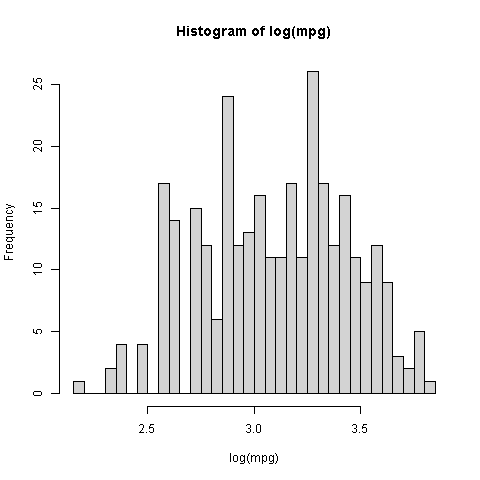
\includegraphics[scale=0.4]{img/mpgloghist.png}
\caption{Histogram of the natural logarithm of mpg}
\label{fig:my_label_with_H}
\end{figure}

\subsubsection{Multicollinearity}

We still haven't discussed the possibility of multicollinearity in our model, for good reasons. Some of our variable can be relate to each other, in a very natural way as they are describing the characteristics of a car. For examples, we can make some guess about their relation:

\begin{itemize}
    \item Displacement and weight: The engine make up a significant portion of a car's weight. As such it's reasonable to assume a car with higher weight tend to have a larger engine.
    \item Weight and acceleration: A car that's heavier is harder to accelerate.
\end{itemize}

As such, we need to consider the possibility of multicollinearity in our model.

To ensure the model is properly specified and functioning correctly, there are tests that can be run for multicollinearity. The variance inflation factor is one such measuring tool. Using variance inflation factors helps to identify the severity of any multicollinearity issues so that the model can be adjusted.

\begin{table}[H]
\centering
\begin{tabular}{rlrrr}
  \hline
 Variable & GVIF & Df & GVIF\verb|^|(1/(2*Df)) \\ 
  \hline
displacement & 10.70 & 1.00 & 3.27 \\ 
weight & 8.04 & 1.00 & 2.83 \\ 
 acceleration & 1.51 & 1.00 & 1.23 \\ 
 model\_year & 1.21 & 1.00 & 1.10 \\ 
 origin & 1.93 & 2.00 & 1.18 \\ 
   \hline
\end{tabular}
\caption{VIF Analysis} 
\label{tab:vif}
\end{table}


\textbf{Interpretation of GVIF Output:}

\begin{itemize}
    \item \textbf{GVIF}: Generalized VIF adjusts the VIF for degrees of freedom. The larger the GVIF, the more multicollinearity there is in the variable.
    \item \textbf{GVIF\^(1/(2*Df))}: This column normalizes GVIF, making it comparable to standard VIF values when Df (degrees of freedom) is greater than 1. This normalized value should be used for interpretation.
\end{itemize}
 
\textbf{Common Thresholds:}

\begin{itemize}
    \item \textbf{GVIF\^(1/(2*Df)) > $\sqrt(5)$}: Suggests moderate multicollinearity.
    \item \textbf{GVIF\^(1/(2*Df)) > $\sqrt(10)$}: Indicates high multicollinearity and might require corrective actions like removing or combining variables.
\end{itemize}

We can see at a glance that displacement have a really high value GVIF\^(1/(2*Df)) > $\sqrt(10)$, this indicate a severe multicollinearity issue in our model. While we still haven't removed this variable yet. This is an important information for later. 

Note: Displacement is going to be removed eventually with the stepwise method. This will solve our multicollinearity problem. We can see this through the VIF analysis of the reduced model without displacement.

\begin{table}[ht]
\centering
\captionof{table}{VIF Analysis of the reduced model}
\begin{tabular}{rrrr}
  \hline
 & GVIF & Df & GVIF\verb|^|(1/(2*Df)) \\ 
  \hline
  weight & 1.78 & 1.00 & 1.34 \\ 
  acceleration & 1.25 & 1.00 & 1.12 \\ 
  model\_year & 1.18 & 1.00 & 1.09 \\ 
  origin & 1.60 & 2.00 & 1.13 \\ 
   \hline
\end{tabular}
\end{table}

So even though we didn't removed displacement now, after we arrived with our improved model, as displacement is no longer included in our final model. Multicollinearity is no longer an issue for our model.

\subsubsection{Displacement statistical significance issues}

As we can see from the summary of our baseline model, displacement may not have a large statistical significance to our model. In addition, Displacement also has a relative high GVIF value. As such, it can be beneficial to try to remove displacement from our model.

This mean we are testing the hypothesis

\begin{center}
    $H_0: \beta_2 = 0$
    \\
    $H_1:\beta_2 \neq 0$
\end{center}

In our baseline model: 

\begin{center}
$
mpg \ = \ \beta_1 \ + \ \beta_2 \ displacement \ + \ \beta_3 \ weight \ + \ \beta_4 \ acceleration \ + \ \beta_5 \ model\_year \ + \ \beta_6 \ origin_2 \ + \ \beta_7 \ origin_3 \ + \ \epsilon
$
\end{center}


To do this we can do a partial F-test on the baseline model and the reduced model:

\begin{center}
$
mpg \ = \ \beta_1 \ + \ \beta_3 \ weight \ + \ \beta_4 \ acceleration \ + \ \beta_5 \ model\_year \ + \ \beta_6 \ origin_2 \ + \ \beta_7 \ origin_3 \ + \ \epsilon
$
\end{center}

The test statistics value we are trying to calculate is 

\begin{center}
    $f \ = \ \frac{(SSE_l-SSE_k)}{k-l} \ \frac{SSE_k}{n-(k+1)}$
\end{center}

With $k = 6$ (number of predictors), $l = 1$ (number of removed predictor), n = number of observations in our dataset. $SSE_l,SSE_k$ is the unexplained variation for the reduced and full model, respectively.

This calculation can be done easily through ANOVA function in R.

\begin{table}[ht]
\centering
\captionof{table}{ANOVA result of the full and reduced model}
\begin{tabular}{lrrrrrr}
  \hline
 & Res.Df & RSS & Df & Sum of Sq & F & Pr($>$F) \\ 
  \hline
1 & 306 & 3559.85 &  &  &  &  \\ 
  2 & 307 & 3601.52 & -1 & -41.67 & 3.58 & 0.0594 \\ 
   \hline
\end{tabular}
\end{table}

The table give us an $f = 3.58$ and corresponding to a p-value of 0.0594.

This mean that we rejected $H_0$ and conclude that displacement has a statistical significance in our dataset and we cannot removed displacement yet. However, this statistical significance is still very small and only barely make the threshold.

\subsubsection{Transformation of weight}

We examine the Box Cox plot of weight:

\begin{figure}[H]
\centering
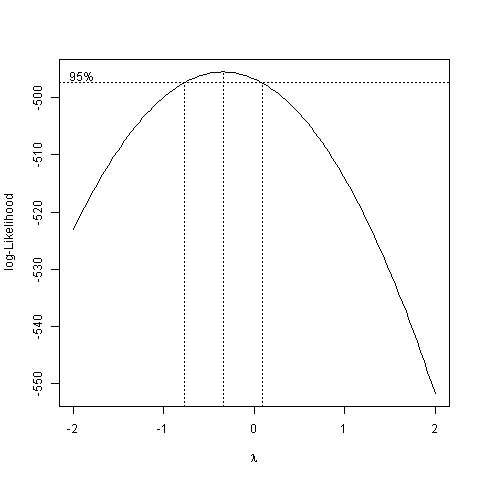
\includegraphics[scale=0.4]{img/weightboxcox.png}
\label{fig:my_label_with_H}
\caption{Box Cox plot of weight}
\end{figure}

The Box Cox plot show us a few way to transform weight.

A simple solution is to take the log of weight. As $\lambda = 0$ is in the range of the confidence interval.

\begin{figure}[H]
\centering
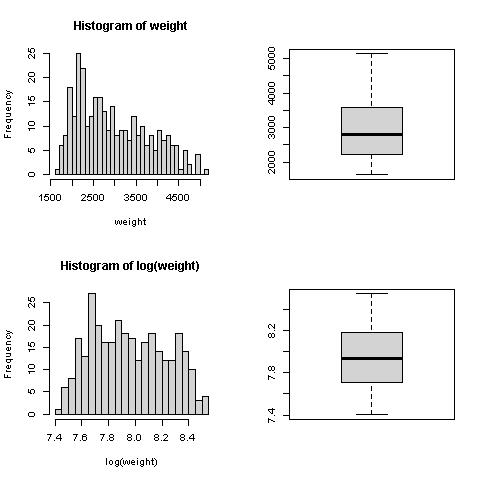
\includegraphics[scale=0.7]{img/weighttrans1.jpeg}
\label{fig:my_label_with_H}
\caption{Histogram and boxplot of weight and log(weight)}
\end{figure}

Another possible path is to take the inverse square root of weight, or $\frac{1}{sqrt(weight)}$ as $\lambda = -0.5$ is also in the interval, or $sqrt(weight)$ as $\lambda = 0.5$ is also pretty close to the confidence inteval.

\begin{figure}[H]
\centering
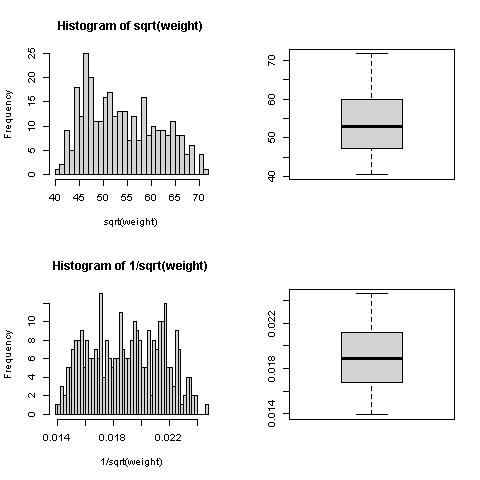
\includegraphics[scale=0.7]{img/weighttrans2.jpeg}
\label{fig:my_label_with_H}
\caption{Histogram and boxplot of sqrt(weight) and $\frac{1}{sqrt(weight)}$}
\end{figure}

We decide to pick log(weight) as it is both simple to implement and having a histogram that pretty close to normal distribution.

\subsubsection{Transformation of acceleration}

We do the same thing as the previous section. We examine the Box Cox plot of acceleration:

\begin{figure}[H]
\centering
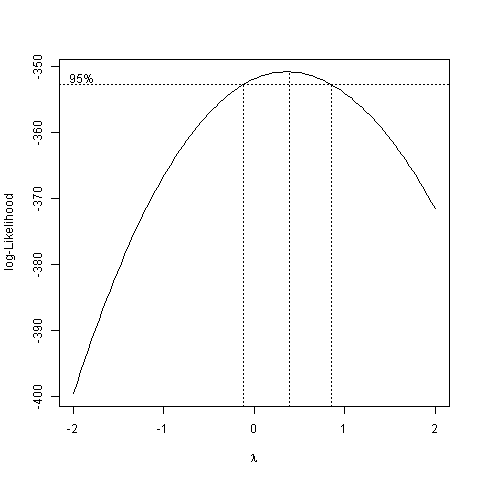
\includegraphics[scale=0.4]{img/accelboxcox.png}
\label{fig:my_label_with_H}
\caption{Box Cox plot of acceleration}
\end{figure}

The Box Cox plot show us a few way to transform acceleration.

A simple solution is to take the log of acceleration. As $\lambda = 0$ is in the range of the confidence interval.

\begin{figure}[H]
\centering
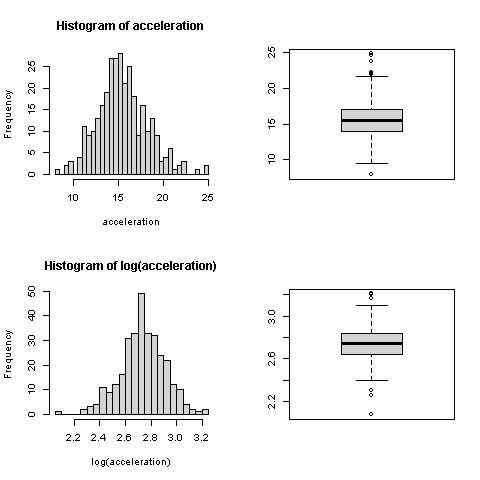
\includegraphics[scale=0.7]{img/acceltrans1.jpeg}
\label{fig:my_label_with_H}
\caption{Histogram and boxplot of acceleration and log(acceleration)}
\end{figure}

Another possible path is to take the inverse sqrt of acceleration, or $\frac{1}{sqrt(acceleration)}$ as $\lambda = -0.5$ is also pretty close to the interval, or sqrt(acceleration) as $\lambda = 0.5$ is in the confidence inteval.

\begin{figure}[H]
\centering
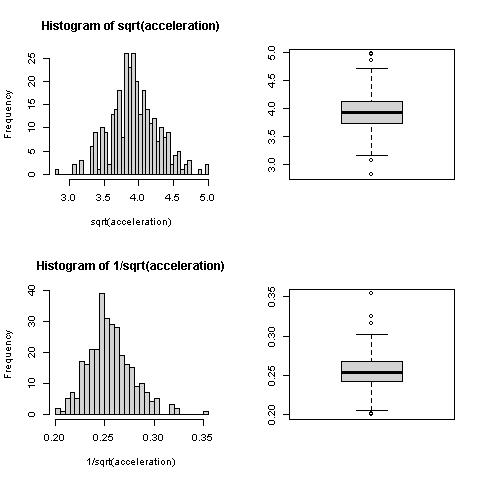
\includegraphics[scale=0.7]{img/acceltrans2.jpeg}
\label{fig:my_label_with_H}
\caption{Histogram and boxplot of sqrt(acceleration) and $\frac{1}{sqrt(acceleration)}$}
\end{figure}

We decide to test both acceleration and log(acceleration).

\subsubsection{Model year as multi-value discrete variable vs. continuous variable}

Here, we are having to make an important decision. Making model year as an multi-value discrete variable or a continuous variable. While model year only take integer value from 70 to 78. We decide to make model year a continuous variable after weighting the pros and cons:

Advantages of making model$\_$year a multi-value discrete variable:
\begin{itemize}
    \item We can make indicator variable for each year, or each group of year. Improving the accuracy of our model.
\end{itemize}

Disadvantages of making model$\_$year a multi-value discrete variable:
\begin{itemize}
    \item Harder to implement, more variable to consider.
    \item Can only be used to estimate car made from 1970 to 1978.
\end{itemize}

Advantages of making model$\_$year a continuous variable:
\begin{itemize}
    \item Easier to implement.
    \item More general, can be use to predict future value, beyond the value of data set provided.
\end{itemize}

Disadvantages of making model$\_$year a continuous variable:
\begin{itemize}
    \item Less accurate, as the rate of change between year may not be linear.
\end{itemize}

In the end, we pick making model$\_$year a continuous variable for generalibilty.

\subsubsection{The improved model}

From various adjustment from the previous sections, we are now left with two model $M_1$ and $M_2$:

\begin{center}
$
M_1: \ log(mpg) \ = \ \beta_1 \ + \ \beta_2 \ displacement \ + \ \beta_3 \ log(weight) \ + \ \beta_4 \ acceleration \ + \ \beta_5 \ model\_year \ + \ \beta_6 \ origin_2 \ + \ \beta_7 \ origin_3 \ + \ \epsilon
$
\end{center}

\begin{center}
$
M_2: \ log(mpg) \ = \ \beta_1 \ + \ \beta_2 \ displacement \ + \ \beta_3 \ log(weight) \ + \ \beta_4 \ log(acceleration) \ + \ \beta_5 \ model\_year \ + \ \beta_6 \ origin_2 \ + \ \beta_7 \ origin_3 \ + \ \epsilon
$
\end{center}

We run the stepwise procedure again on these model and obtain our result, let's called these result $M_1'$ and $M_2'$.

\begin{center}
$
M_1': \ log(mpg) \ = \ \beta_1 \ + \ \beta_3 \ log(weight) \ + \ \beta_4 \ acceleration \ + \ \beta_5 \ model\_year \ + \ \beta_6 \ origin_2 \ + \ \beta_7 \ origin_3 \ + \ \epsilon
$
\end{center}

\begin{center}
$
M_2': \ log(mpg) \ = \ \beta_1 \ + \ \beta_3 \ log(weight) \ + \ \beta_4 \ log(acceleration) \ + \ \beta_5 \ model\_year \ + \ \beta_6 \ origin_2 \ + \ \beta_7 \ origin_3 \ + \ \epsilon
$
\end{center}

So both come to the conclusion to exclude displacement from the model, this is expected as from the previous section, displacement is a candidate for multicollinearity and does not have a large statistical significance to our model.

We also get the evaluation parameter of these two model.

\begin{table}[H]
\centering
\captionof{table}{Evaluation parameter of $M_1'$ and $M_2'$}
\begin{tabular}{rll}
  \hline
               & $M_1'$             & $M_2'$    \\
    \hline
$R^2$          & \textbf{0.8842}    & 0.8837    \\
Adjusted $R^2$ & \textbf{0.8823}    & 0.8818    \\
AIC            & \textbf{-443.8934} & -442.4572 \\
BIC            & \textbf{-417.67}   & -416.2338 \\
   \hline
\end{tabular}
\label{tab:vif}
\end{table}

This show that $M_1'$ is the superior model, as such we take $M_1'$ as our final model.

\subsection{Hypothesis testing}

Before proceeding, we rewrite our model a little bit:

\begin{center}
$
M: \ log(mpg) \ = \ \beta_1 \ + \ \beta_2 \ log(weight) \ + \ \beta_3 \ acceleration \ + \ \beta_4 \ model\_year \ + \ \beta_5 \ origin_2 \ + \ \beta_6 \ origin_3 \ + \ \epsilon
$
\end{center}

\subsubsection{Model utility}

We are testing the hypothesis:

\begin{center}
    $H_0: \beta_i = 0, i \in \{2,3,4,5,6\}$
    $ \\ $
    $H_1:$ At least one of $\beta_i \neq 0, i \in \{2,3,4,5,6\}$
\end{center}

This mean we are calculating the test statistic value $f= \frac{R^2/k}{1-R^2} \ \frac{1}{(n-(k+1)}$.

Plugging in the number we get $f = 468.8$, this corresponding to a p-value of $2,2.10^{-16}$. This mean we can be certain to reject $H_0$. And conclude that our model contains useful linear relationship between our the response mpg and at least one of the variable.

\subsubsection{Predictor statistical significance}

This mean, for each $i \in \{2,3,4,5,6\}$. We are testing the hypothesis.


\begin{center}
    $H_0: \beta_i = 0$
    \\
    $H_1:\beta_i \neq 0$
\end{center}

To do this we can do a partial F-test on the reduced model and our full model. This is similar to the method describe in a previous section.

Again, this can be easily done with the ANOVA function in R. Here are the result for each partial F-test for each variables:

\begin{table}[ht]
\centering
\begin{tabular}{rrrrr}
  \hline
 & f & P-value \\ 
  \hline
  log(weight) & -27.00 & 0.0000 \\ 
  acceleration &  2.37 & 0.0182 \\ 
  model\_year & 17.33 & 0.0000 \\ 
  origin2 & 3.33 & 0.0010 \\ 
  origin3 & 1.54 & 0.1253 \\ 
   \hline
\end{tabular}
\end{table}

The only variable that failed this test is the origin3, or that's mean we failed to reject the hypothesis that $\beta_6 = 0$. However, let's consider the evaluation parameter of the reduced model (the model without origin 3:

\begin{table}[H]
\centering
\captionof{table}{Evaluation parameter of full and reduced}
\begin{tabular}{rll}
  \hline
               & Full model             & Reduced model    \\
    \hline
$R^2$          & \textbf{0.8842}    & 0.8837    \\
Adjusted $R^2$ & \textbf{0.8823}    & 0.8818    \\
AIC            & \textbf{-443.8934} & -442.4572 \\
BIC            & \textbf{-417.67}   & -416.2338 \\
   \hline
\end{tabular}
\label{tab:vif}
\end{table}

We can see that removing origin3 does not neccessary improve our model. In addition, removing origin3 mean that the user need to do an additional layer of preprocessing when using our model. Hence, we decided to keep origin3.

\subsubsection{Error normality assumption}

We are testing the hypothesis of:

\begin{center}
    $H_0: \epsilon$ is normal distributed
    \\
    $H_1:\epsilon$ is not normal distributed
\end{center}

To test this, we can use the test data. Let's predict$\_$mpg be our result after passing the test observation through the model. Let's mpg be the corresponding value of that observation. Then, $\epsilon = predict\_mpg - mpg$. We will run the Shapiro-Wilk test through this resulting error.

Here the result of our Shapiro-Wilk test:

\begin{table}[H]
\centering
\captionof{table}{Shapiro-Wilk test result}
\begin{tabular}{ll}
  \hline
                W             & p-value    \\
    \hline
        0.97088    & 0.06765   \\

   \hline
\end{tabular}
\label{tab:vif}
\end{table}

This mean we have failed to reject the hypothesis that $\epsilon$ is normal distributed. 

\subsubsection{Homoskedastic residual variance}

Here we are testing the hypothesis of:

\begin{center}
    $H_0:$ The residuals variances of the groups are equal.
    \\
    $H_1:$ At least one group has a different residuals variance.
\end{center}

To test this, we can run the Levene's test, which is available in R. After running the test, we get the result:

\begin{table}[H]
\centering
\captionof{table}{Levene test result}
\begin{tabular}{ll}
  \hline
                F             & p-value    \\
    \hline
        2.7299 &  0.0668   \\

   \hline
\end{tabular}
\label{tab:vif}
\end{table}

This mean we have failed to reject the null hypothesis. This indicate that the residuals variances of the groups are equal.

\subsubsection{Autocorrelation}

We are testing the hypothesis:

\begin{center}
    $H_0:$ There is no autocorrelation in the error terms of the linear regression model.
    \\
    $H_1:$ There is positive autocorrelation in the error terms of the linear regression model.
\end{center}

To test this, we can run the Durbin-Watson test, which is available in R. After running the test, we get the result:

\begin{table}[H]
\centering
\captionof{table}{Durbin-Watson test result}
\begin{tabular}{ll}
  \hline
                D-W             & p-value    \\
    \hline
        1.950639  & 0.668   \\

   \hline
\end{tabular}
\label{tab:vif}
\end{table}

This mean we have failed to reject the null hypothesis. This indicate that there is no autocorrelation in the error terms of the linear regression model.

\subsection{Validation and testing}

We used the same definition of predict$\_$mpg as the previous section. It's the result of passing the test data through our model.

Here is the histogram of predict$\_$log(mpg):


\begin{figure}[H]
\centering
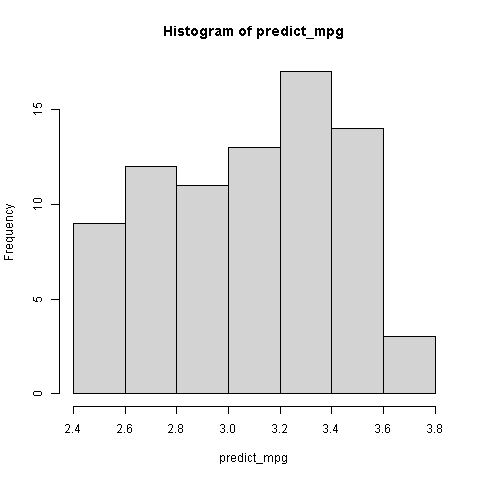
\includegraphics[width=0.55\textwidth]{img/predictmpghist1.png}
\caption{Prediction of log(mpg)}
\label{fig:scaled_revenue_distribution}
\end{figure}

As our model estimate log(mpg), we have to take this to the power of e in order to be comparable to mpg. After taking predict$\_$mpg to the power of e. Here is the histogram of it:

\begin{figure}[H]
\centering
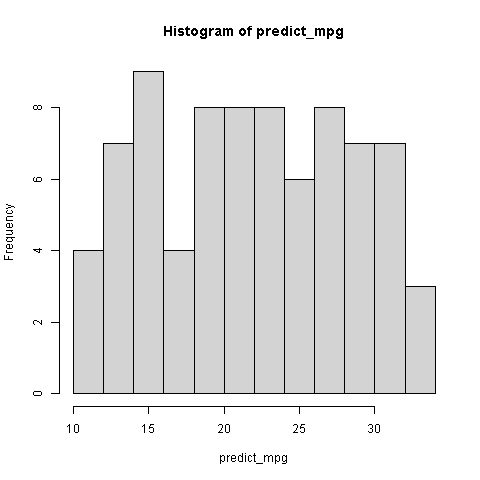
\includegraphics[width=0.55\textwidth]{img/predictmpghist2.png}
\caption{Prediction of mpg}
\label{fig:scaled_revenue_distribution}
\end{figure}

We compare this to the actual value of mpg, here is the scatter plot of them:

\begin{figure}[H]
\centering
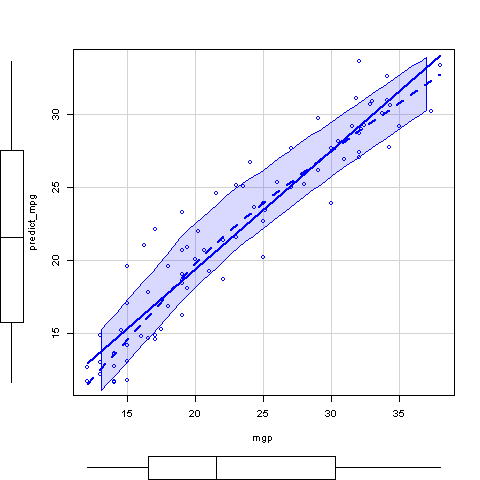
\includegraphics[width=0.55\textwidth]{img/mpgpredict.png}
\caption{Histogram of actual mpg}
\label{fig:scaled_revenue_distribution}
\end{figure}

As they form a almost 45 degree line in the diagonal of the graph, we can say that our model have predict the value of mpg pretty closely.

\subsection{Model meaning}

Our model is capable of estimating the fuel efficiency of car model with 4 parameter: weight, acceleration, model$\_$year and origin. As model$\_$ year is used as a continuous variable, this model can also be used for future car model, though in that case, we may need to reexamine the accuracy of the model.

Overall, Here is our final model:

\begin{center}
$
M: \ log(mpg) \ = \ \beta_1 \ + \ \beta_2 \ log(weight) \ + \ \beta_3 \ acceleration \ + \ \beta_4 \ model\_year \ + \ \beta_5 \ origin_2 \ + \ \beta_6 \ origin_3 \ + \ \epsilon
$
\end{center}

With:

\begin{center}
    $\beta_1 = 7.375331$
    $\beta_2 = -0.874849$
    $\beta_3 = 0.006518$
    $\beta_4 = 0.033764$
    $\beta_5 = 0.069592$
    $\beta_6 = 0.031755$
\end{center}

Variable meaning:

\begin{itemize}
    \item mpg: Fuel efficiency, calculated as miles per gallon (mpg)
    \item weight: Car weight (lbs)
    \item acceleration: Car's acceleration (ft/$s^2$)
    \item model$\_$year: Number of year after 1900 that the car is manufactured.
    \item origin2: 1 if manufactured in Europe, 0 otherwise.
    \item origin3: 1 if manufactured in Asia, 0 otherwise.
\end{itemize}

This mean that:

\begin{itemize}
    \item The initial log(mpg) of a car is 7.375331. Which equate to 228.5 miles per gallon.
    \item When log(weight) increase by 1, the log(mpg) decrease by -0.874849.
    \item When acceleration increase by 1 unit, log(mpg) increase by 0.006518
    \item For a car that is built one year later than another, it's log(mpg) is increase by 0.033764.
    \item A car built at Europe has its log(mpg) 0.069592 unit higher than a car built at North America.
    \item A car built at Asia has its log(mpg) 0.031755 unit higher than a car built at North America.
    \item This assume all other variable is the same.
\end{itemize}

In layman's terms, this mean:

\begin{itemize}
    \item The heavier the car, the less fuel efficient it is.
    \item The faster the car can accelerate, the more fuel efficient it is.
    \item Car are more fuel efficient in the future than in the past.
    \item Car built at Europe is more fuel efficient than the same car built at Asia, which is also more fuel efficient than the same car built at North America.
\end{itemize}

Please note these are infer from the data set and may not truly represent the real world. However, in the scope of our data set, our model have accurately estimate the fuel efficiency of the car, given the data. It also show potential to be used to estimate cars which are made beyond 1978, which is the limit of the data set.